
\chapter{Speaker Diarization in Co-channel Speech}
\label{chap:spkr_diar}

Throughout the course of this study, part of the agenda has been to acknowledge non-overlapping speech as an important component of co-channel. 
It was shown that distinguishing overlap from co-channel introduces more realistic scenarios to the scope of co-channel speech problems. 
An important example of such kinds of problem is conversational speech, a common and realistic form of speech. 
Among the various aspects of analyzing conversations, {\it speaker diarization} is closest to speaker recognition\footnote{As a reminder for the readers, speaker recognition is the main theme of this thesis.}.
Speaker diarization refers to the task of automatically determining ``who spoke when?'' within an audio signal containing two or more speakers. 
This chapter addresses the tasks of 1) segmenting co-channel data into single-speaker excerpts and 2) clustering segments, which means to group them by speakers. 
Tasks are described within the context of CRSSDiar, a speaker diarization tool-kit designed to perform diarization while simultaneously supporting speaker recognition and speech recognition using Kaldi\cite{kaldi}. 
Therefore, the contribution of this chapter is an end-to-end conversation analysis research platform that is tightly connected to Kaldi and does not require cross-platform coding interfaces. 

CRSSDiar is a speaker diarization tool-kit developed as part of a collaboration between myself and Chengzhu Yu, a fellow PhD student at the Center for Robust Speech Systems (CRSS). 
The main motivation behind developing this tool-kit is to establish an integrated end-to-end conversation analysis system that provides the capability of diarizing  signals while supporting speech recognition. 
Currently, one of the most popular speech recognition platforms used in research is Kaldi, developed in Johns Hopkins University~\cite{kaldi}. 
Existing diarization systems are implemented in different platforms and to the best of our knowledge none support Kaldi I/O functions. 
Switching between platforms and APIs\footnote{Application Programming Interface} frustrates users who are interested in simultaneously analyzing speaker diarization and speech recognition. 
We hope that developing a speaker diarization module on top of Kaldi will help students and staff with the kind of multi-purpose research that is common in CRSS. 
Although CRSSDiar is currently in working condition, as a research platform it is always considered under development and is available for those who are interested in investigating various aspects of conversational data. 
In Sect.~\ref{sec:crssdiar_layout}, a layout of the system and its relationship with Kaldi is presented. 
Section~\ref{sec:crssdiar_layout} also provides a list of our modules and their Input/Output. 
I also explain how these modules interact with Kaldi data types. 
In Sect.~\ref{sec:segmentation}, segmentation, the first task of speaker diarization, is described. 
The purpose of segmentation is to split signals into smaller chunks that contain only one speaker. 
Some segments may contain overlapped speech or no speech at all. 
Therefore, as part of segmentation, speech activity detection (SAD) and overlap detection modules are also integrated into the system. 
In Sect.~\ref{sec:clustering}, the clustering (grouping) module is presented. 
A state-of-the-art technique, called integer linear programming (ILP), is used in CRSSDiar to cluster segments obtained from the segmentation stage~\cite{bredin2013ILP}. 
Clustered groups represent segments that belong to the same speaker. Another component also described in Sect.~\ref{sec:clustering} is the re-segmentation, which acts as a correction layer on top of the clustering module. 

Part of the reason this chapter is placed at the end of the dissertation is that it can be viewed as a description of a comprehensive system that contains all of the problems we have looked at so far. 
Furthermore, since CRSSDiar is a research platform that could potentially benefit those looking beyond the scope of this study, I consider it a gateway to future work for my thesis. 



 
\section{CRSSDiar Layout}
\label{sec:crssdiar_layout}

The approach in speaker diarization is to split an audio recording (usually at least a few minutes long) into smaller segments that only contain one speaker.
After completing the first step, one must label the segments according to speaker identities. 
The assumption is that no prior knowledge of the number of speakers or their identities is available. 
The only possible solution, therefore, is to compare the segments and group those that appear to belong to the same speaker. 

The segment-and-cluster approach is the most common solution to speaker diarization~\cite{meignier2010lium,anguera2012diarization}. 
That being said, alternative approaches have been proposed. 
Especially, with regard to segmentation and post-clustering steps. 
Some studies completely ignore the segmentation step and use equal-length segments to perform clustering~\cite{sell_garcia_2015diarization}. 
Skipping segmentation is an attractive proposition, since as we will see in the following section, segmentation is prone to errors. 
In addition, using equal lengths instead of varying-length segments to some extent guarantees equal reliability of individual segments for the clustering step. 
We say equally reliable because speaker-dependent features (e.g. i-vectors) are known to depend largely on the length of the signals~\cite{hasan2013duration} from which they are extracted. 
When automatic segmentation is used to split the audio recording, segments lengths may vary causing the corresponding speaker-dependent features to vary in quality and reliability. 

Another component of speaker diarization, not mentioned above, is the re-segmentation step. 
Re-segmentation is a post-clustering step used to prevent sudden changes in the speaker. 
The reason this module is important is the fact that clustering does not take time sequences into account when grouping segments. 
Meanwhile, as listeners we expect a certain amount of coherence in conversations. 
This presumed coherence in the sequence of speakers is used to correct errors in the clustering step. 

Figure~\ref{fig:crssdiar} shows an overview of CRSSDiar. 
The input is the audio recording of two or more speakers. 
We start by performing speech activity detection (SAD) and overlap detection to label non-speech and overlapped segments as off-bounds. 
The next step is segmentation, which uses a measure called Bayesian Information Criterion (BIC) to detect speaker change points~\cite{chen1998BIC}. 
After BIC-Segmentation, we have access to segments within the audio recordings and would like to label these segments to determine which belongs to which speaker (speaker A, B, C, etc.). 
Of course, these speaker identities are assigned relative to the input audio and are not actual speaker identities. 
This means that given another input signal, the speaker diarization system will provide similar labels, but speaker A in audio 1 has no relation to speaker A in audio 2. 
CRSSDiar generates speaker labels using integer linear programming (ILP) to cluster the segments. 
ILP, described in detail in Sect.~\ref{sec:clustering}, uses a global optimization approach to minimize speaker diversity within each cluster while simultaneously minimizing the number of clusters (aka speakers). 

Thus is the overview of a standard speaker diarization system. 
As mentioned before, there are many implementations available for speaker diarization. 
What CRSSDiar offers in addition is to allow speaker diarization in a platform that also supports speech and speaker recognition (Kaldi). 


\begin{figure}[t!]
	\centering
	\textbf{Speaker diarization system description}\par\medskip
	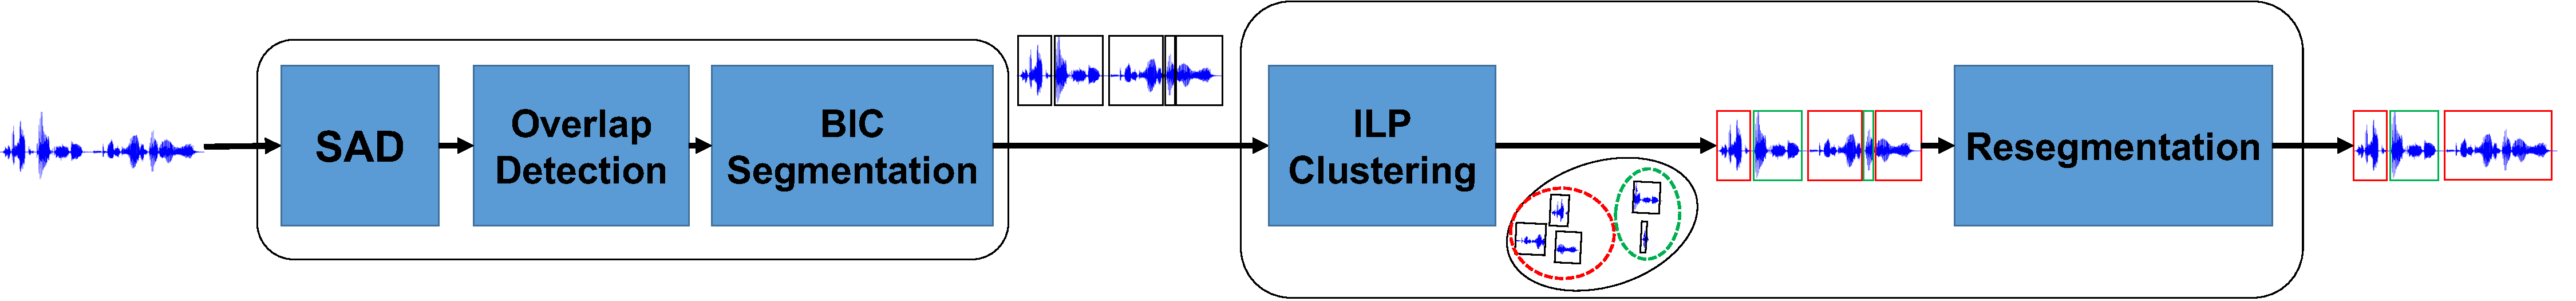
\includegraphics[height = 1in, width=1\textwidth]{figures/crssdiar_outline}
	\caption{\it \small CRSSDiar system overview. Two main steps are used in speaker diarization: 1) Segmentation (SAD, overlap detection, and BIC segmentation) and 2) clustering (ILP clustering and resegmentation). }
	\label{fig:crssdiar}
	\vspace{-3mm}
\end{figure}

\subsection{Interaction with Kaldi}
\label{ssec:crssdiar_and_kaldi}

As pointed at the beginning of the chapter, a driving force in developing this tool-kit was high compatibility with the Kaldi speech and speaker recognition platform~\cite{kaldi}. 
For those not familiar with the Kaldi project, it is a toolkit for speech recognition written in C++ and licensed under the Apache License v2.0. Kaldi is intended for use by speech recognition researchers~\cite{kaldi}. 
Kaldi comprises many modules each designated to a specific task. For example, {\it feat} for feature extraction or {\it ivector} for ivector-based speaker recognition. 
Most modules come with a corresponding {\it bin} directory  that contains executable files used to perform various functions in a speech or speaker recognition system (e.g. {\it featbin}, {\it ivectorbin}). 
The executables are those most users interact with in their Bash scripts. These Bash scripts are also referred to as ``recipes''. 
CRSSDiar follows the same convention and consists of a {\it diar} and a {\it diarbin} directory. 
The classes are defined in {\it diar}, while {\it diarbin} contains the executables used to perform segmentation and clustering. 
CRSSDiar uses matrix and utility libraries from Kaldi in its core.  
Kaldi also includes modules that define Gaussian mixture models and Hidden Markov models ({\it gmm} and {\it hmm}), of which we also take advantage for acoustic modeling. 
As mentioned in the previous section, i-vectors are used in CRSSDiar as speaker-dependent features. 
Therefore, Kaldi's {\it ivector} is used to extract i-vectors and calculate distances and models such as PLDA\footnote{probabilistic linear discriminant analysis} to perform clustering. 
Figure~\ref{fig:crssdiar_vs_kaldi} shows the interaction between {\it diar} and {\it diarbin} components and Kaldi libraries. 

\begin{figure}[t!]
	\centering
	\textbf{CRSSDiar modules}\par\medskip
	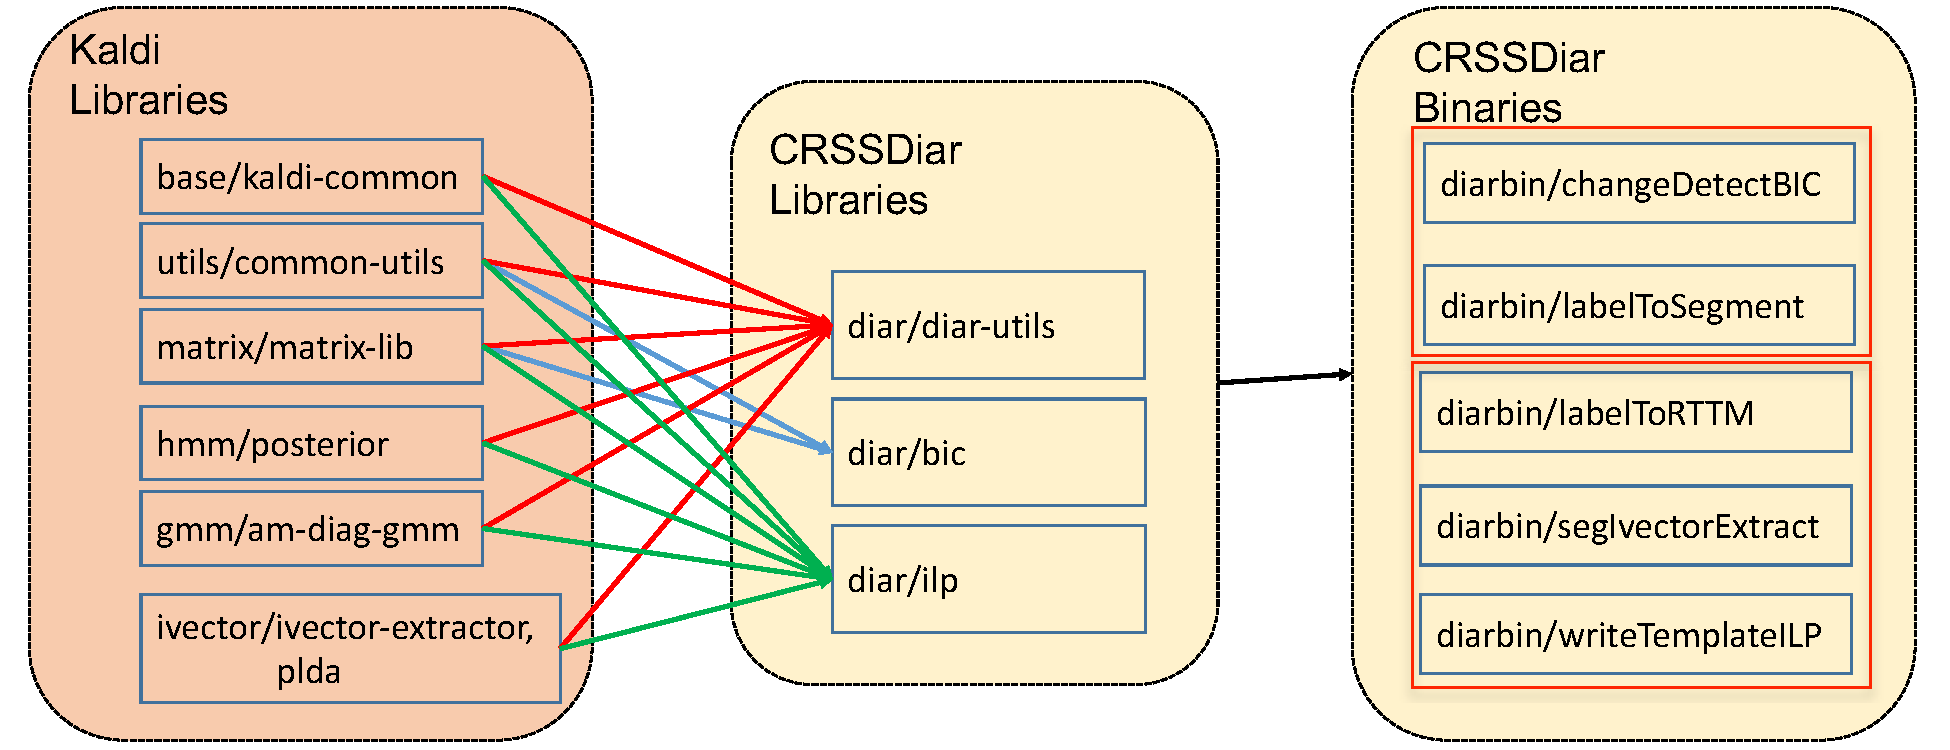
\includegraphics[height = 2in, width=0.8\textwidth]{figures/crssdiar_and_kaldi}
	\caption{\it \small CRSSDiar components and their relation with Kaldi libraries.  }
	\label{fig:crssdiar_vs_kaldi}
	\vspace{-3mm}
\end{figure}

\section{Segmentation}
\label{sec:segmentation}
This section briefly describes the layout of the Segmentation component in CRSSDiar. 
Traditionally, the approach for speaker diarization has been to first identify speaker change points in an audio stream. 
This is due to the restrictive framework of typical speaker diarization problems. 
The restriction being no prior knowledge of the number or identity of the speakers in the signal. 
Therefore, the solution is to track acoustic features along the signal and detect points at which these features demonstrate significant changes. 

Segmentation in the context of this study is formally defined as detecting the time indexes corresponding to changes in an ordered sequence of acoustic features~\cite{cettolo2005evaluation}. 
One of the most popular speaker change detection algorithms used in speaker diarization is the Bayesian information criterion (BIC), which is briefly described in this section. 
I should point out that BIC segmentation has been thoroughly studied in the research community and several resources are available that substantially cover the essentials required to understand its function in a speaker diarization system~\cite{cettolo2003efficient,cettolo2005evaluation,chen1998BIC}. 
The content here is intended to describe all aspects of CRSSDiar and share implementation details for the curious reader. 

\subsection{Bayesian Information Criterion}
\label{ssec:chDiar_secBIC}
The Bayesian information criterion (BIC) is a measure that determines the effectiveness of a given probabilistic model in capturing statistical characteristics of a set of data samples. 
BIC is used in segmentation as a way to quantify the certainty of the existence of a break-point in a given window of the audio. 
Therefore, instead of finding a global solution to the segmentation problem defined in Sect.~\ref{sec:segmentation}, the standard BIC implementation tracks a sliding window in the audio and compares the compares the following two hypotheses: 
\begin{itemize}
	\item $H_0$: The window does not contain a breaking point. 
	\item $H_1$: The window contains exactly one breaking point. 
\end{itemize}

In speaker diarization terms, $H_0$ implies that the window contains one speaker, while $H_1$ implies that two speakers exist. 
BIC segmentation tests these hypotheses by using the following function in a sequence of acoustic features in a window, $\{X_1X_2...X_N\}$, for the hypothesis $H$:
\begin{equation}
BIC(H) = log\mathcal{L}_{M}(H) - P_{M_{N}}, 
\end{equation}
where $\mathcal{L}_{M}(H)$ is the maximum likelihood of the model $M$ under hypothesis $H$. $P_M$ is the BIC penalty function~\cite{schwarz1978BIC} when $M$ is used to parameterize $N$ samples. The indexes correspond to time frames\footnote{As we know, acoustic features, $X_i$, are calculated over typically $25 msec$ frames. 
The framing used throughout this chapter uses $25 msec$ frames with an increment of $10 msec$. These frames are not to be mistaken with windows used to search for change points.}. 
\begin{equation}
P_{M_N} = \frac{F_M}{2}log(N),
\end{equation}
with $F_M$ as the degrees of freedom of the chosen model, $M$. 
When the sequence $\{X_1X_2...X_N\}$ comprises two segments (i.e., $H = H_1$), the break-point is assumed to be an index $i_{max}$ between $1$ and $N$. 
$BIC(H_1)$ is maximized at the break-point $i = i_{max}$. 
This assumption states that breaking the sequence into two sub-sequences $\{X_1X_2...X_{i_{max}}\}$ and $\{X_{i_{max}+1}X_{i_{max}+2}...X_N\}$ maximizes the BIC penalty. 
On the other, if the sequence does not contain a break-point (i.e., $H_0$), $i_{max}$ can be assumed equal to $N$. 
The actual measure used in BIC segmentation is the difference between the BIC corresponding to $H_0$ and the BIC of $H_1$. This value is called $\Delta BIC_i$: 
\begin{equation}
\Delta BIC_i = (log \mathcal{L}_{M_i} - P_{M_i}) - (log \mathcal{L}_{M_N} - P_{M_N})
\end{equation}
where $\mathcal{L}_{M_i}$ is short-hand for the maximum likelihood of $H_1$ when the break-point is at index $i$. 
If $\Delta BIC_i > 0$, the model favors $H_1$ and otherwise the model suggests no break-points ($H_0$).  

$\Delta BIC$ Depends on the model chosen for $M$. 
A common choice in speaker diarization is a Gaussian model, which investigates whether the sequence is best described with one covariance matrix ($H_0$) or two ($H_1$). 
In~\cite{cettolo2005evaluation}, $\Delta BIC_i$ is derived for Gaussian modeling with the inclusion of a sensitivity factor $\lambda$. 
\begin{equation}
\label{eq:dbic_gaussian}
\Delta BIC_i = \frac{N}{2} log |\Sigma| - \frac{i}{2} log |\Sigma_1| - \frac{N-i}{2}log |\Sigma_2]| - \lambda P_{M_N}
\end{equation}
where $\Sigma$ is the maximum likelihood estimate of the covariance matrix of $\{X_1X_2...X_N\}$. Similarly, $\Sigma_1$ corresponds to the sequence $\{X_1X_2...X_i\}$ and $\Sigma_2$ to $\{X_{i+1}X_{i+2}...X_N\}$. 
$P_M$ in (\ref{eq:dbic_gaussian}) is the BIC penalty of modeling $N$ samples with a Gaussian. 
The number of free parameters in a multi-variate Gaussian is $d + \frac{d(d+1)}{2}$, in which $d$ is the dimension of the acoustic features. 
The degrees of freedom include $d$ values for the Gaussian mean and $\frac{d(d+1)}{2}$ values for the symmetric covariance matrix. 

In addition to identifying whether a window contains one or two speakers, the segmentation module is also expected to return a time index for the change point. 
BIC segmentation returns this value by incrementally increasing the index $i$ until the point at which $\Delta BIC_i$ is positive. 
Once the change point is detected, granted that it exists in the first place, a recursive search is conducted with smaller increments to find the exact change point. 

Now that the background theory of BIC segmentation has been presented, we move on to a description of BIC segmentation in CRSSDiar in a module called change-point detection. 

\subsection{Change-Point Detection in CRSSDiar}
Change-point detection, or change detection in short, is a tool used to estimate segment boundaries in an audio stream. 
It performs BIC segmentation on speech segments produced from speech activity and overlap detection. 
From here on speech segments refer to segments that may contain multiple non-overlapping speakers or a single speaker. 
The no-overlapping property is implied unless ``overlapped segments'' is used. 
The goal is to split segments at locations where speakers change. 
There is no prior assumption regarding the number of speakers in any given segment. 
The output of change detection, however, will ideally produce smaller segments that each of which contains only one speaker. 

Given a segment, change detection first examines whether the segment is long enough to sufficiently reliable BIC estimates (as defined in Sect.\ref{ssec:chDiar_secBIC}). 
For segments that are sufficiently long, a sliding window is defined that incrementally grows in size. 
This window will grow until: 1) either a change point is detected using the $\Delta BIC$ measure from (\ref{eq:dbic_gaussian}) or 2) the length of the window reaches a maximum acceptable length at which point the window is assumed to contain only one speaker (no change points are detected). 
As mentioned, the window slides until it reaches the end of the segment and returns the change points that were found during the search. 

Every time a change point is detect the window first performs an identical search with more refined search increments until it finds the feature index, $i$, at which $\Delta BIC_i$ is maximized. 
After finding $i_{max}$, the window is reset and continues the search at $i_{max}+1$. 

Figure~\ref{alg:changedetection} shows the pseudo-code for change detection. 
The algorithm requires a set of user defined parameters that determine the search speed and BIC sensitivity. 
\begin{itemize}
	\item $N_{min}$: minimum window length (in number of frames) used to start search for change point. Segments shorter than this value are not sufficiently long to estimate $\Delta BIC$. 
	\item $N_{max}$: maximum window length. The search window grows incrementally until it reaches this maximum length. If the search window reaches this value before a change point is detected, the algorithm quits the search and declares no change point. 
	\item $N_{margin}$: window margin. These margins are used to assure that sufficient number of 
	\item $N_{second}$: refining window length. Once a change-point is detected, the search is refined using a smaller window of this length. 
	\item $N_{shift}$: sliding parameter. The window slides to the right once its length reaches $N_{max}$. 
	\item $N_{grow}$: The incremental growth factor. Every time a window is examined for change points, the window length increases by $N_{grow}$.
	\item $\lambda$: BIC sensitivity factor. The higher this value, the more sensitive $\Delta BIC$ to changes. 
	\item $lowResolution$: initial search increment used to calculate $\Delta BIC_i$. The value $i$ increments by $lowResolution$ in each iteration.
	\item $highResolution$: refined search increment. After a change point is detected in the initial search, a second search window is created and search with an increment of $highResolution$. 
\end{itemize}

\begin{figure}
\begin{lstlisting}
SplitSegment
// Perform BIC change dectect on single speech segment.
if (Nmin >= segment.Length) 
	return
window.Create(segment.Start + Nmargin,Nmin)

while (window.End <= segment.End) 
	maxBICIndexValue = DeltaBIC(window, lowResolution)
	while (maxBICIndexValue <= 0 & window.Length < Nmax) & window.End <= segment.End) 
		window.GrowWindow(Ngrow)
		maxBICIndexValue = DeltaBIC(window,lowResolution)
		
	while (maxBICIndexValue <= 0 & window.End <= segment.End) 
		window.ShiftWindow(Nshift)
		maxBICIndexValue = DeltaBIC(window,lowResolution);
	
if (maxBICIndexValue.second > 0  & window.End <= segment.End) 
	window.Restart(Nsecond)
	maxBICIndexValueHighRes = DeltaBIC(window, highResolution)
	if (maxBICIndexValueHighRes.second > 0) 
		i_max = maxBICIndexValueHighRes.Index
		bicSegments.Create([segment.Begin,i_max]);
		segment.Begin = i_max + 1;
		window.ResetWindow(segment.Begin,Nmin);
else 
	window.ResetWindow(segment.End - Nmargin + 1, Nmin)
\end{lstlisting}
\caption{Algorithm - change detection using BIC. The algorithm describes the two-step procedure of searching for change points in an audio segment. The first step is to search for change points using larger increments, $lowResolution$. Once the change point is detected, a second, more refined, search is performed in a smaller search window using $highResolution$.}
\label{alg:changedetection}
\end{figure}

An important component of change detection is the {\it segment} data type. 
This class contains all the necessary information to calculate functions used in speaker diarization. 
For example, each {\it segment} contains to variable {\it Begin} and {\it End} that indicate the start and end frames corresponding to that segment. 
This class also includes functions used to calculate i-vectors, which will be used extensively in the next section. 
Segments is considered the core data type used in CRSSDiar and is highly compatible with existing Kaldi classes. 

\newpage
\section{Clustering}
\label{sec:clustering}
This section describes the second step in speaker diarization, clustering the segments. 
After single-speaker segments are identified, the speaker diarization system must decide which segments belong to the same speaker. 
This is accomplished without prior knowledge of the number of speakers or their identities. 
The task of grouping segments that belong to the same speaker is known as clustering. 

A number of bottom-up and top-down solutions have been suggested for the clustering step in speaker diarization~\cite{tranterreynolds2006drzoverview,anguera2012DRZreview}. 
Top-down approaches start by assuming all segments belong to a single cluster and iteratively split clusters into smaller more exclusive groups. 
Bottom-up clustering, on the other hand, starts by assuming each sample is a separate cluster and iteratively merges clusters into more inclusive groups. 
The most popular of these is a bottom-up algorithms called hierarchical agglomerative clustering (HAC). 
This approach first assumes that all segments belong to a separate cluster (i.e., speaker) and iteratively merges the two closest clusters. 
A similarity criterion is used to measure the distance between clusters. 
Performance varies depending on the criterion used (e.g., BIC, Kullback-Leibler divergence). 
This iterative process continues until the similarity criterion is no longer satisfied between any two clusters. 
As opposed to the single multivariate Gaussian used to detect change points in the previous section, the clustering process usually uses more sophisticated measures. 
Gaussian mixture models (GMM) have been proven effective in modeling clusters~\cite{zelenak2010albayzin}. 
As clusters merge, the amount of data available to estimate GMM parameters increases. 
Therefore, GMM reliability increases in HAC iterations. 
It is easy to see why using GMMs was not feasible in the segmentation step, since the amount of data was too little to model an entire GMM. 

Despite its popularity, HAC is associated with a number of issues. 
The most important being the error-propagation that occurs during iterations. 
If two segments are incorrectly grouped together in one iteration, the model (e.g., GMM) used to represent the cluster for the next iteration will not accurately represent the speaker identity, and so on. 
This issue has led many to use other top-down clustering approaches, which are less likely to suffer from error-propagation. Examples being K-means~\cite{shum2011exploiting} or spectral clustering~\cite{shum2012spectralclustering, ning2006spectral}. 
To the best of our knowledge, there are no conclusive results that suggest one clustering method over all others for speaker diarization. 
Another important development with regard to clustering has been to use i-vectors to perform clustering. 
The standard HAC-GMM framework does not use i-vectors in the clustering process. 
Some developments have been made to use i-vector distances in an HAC clustering solution~\cite{}. 
The reader should be reminded that the compatibility of CRSSDiar with Kaldi allows for a complete integration of i-vectors with clustering. 

However, an increasingly popular algorithm that has been used in speaker diarization has been {\it integer linear programming} (ILP). 
Two reasons that make ILP particularly interesting are: 
\begin{itemize}
	\item Given appropriate formulation, ILP can result in global optimum for some clustering problems. 
	\item A vast bed of research exists for linear programming algorithms. Integrating these solutions into any problem, in this case speaker diarization, provides new insights and advantages. 
\end{itemize}

ILP was introduced as a global optimization solution for the clustering problem in speaker diarization by Rouvier and Meignier~\cite{rouvier2012global}. 
An attractive aspect of ILP for speaker diarization is that it is relatively strait-forward to perform ILP clustering on i-vectors~\cite{dupuy2012ivectorsILP}. 
The implementation in CRSSDiar is based on improvements on the original ILP formulation for speaker diarization~\cite{dupuy2014ILPimprovement}. 

The single-speaker segments from change detection can be used to derive i-vectors. 
As you may recall from Chapter~\ref{chapter:backend}, i-vectors are fixed-length vectors that represent speaker-specific characteristic of a given audio signal of variable length. 
ILP is a constrained optimization problem that determines which i-vectors should fall in the same cluster. 
The optimization ensures that:
\begin{enumerate}
	\item all i-vectors in a cluster are within a predefined distance, $\delta$, of all the other i-vectors in that cluster. 
	\item the number of clusters is minimal. 
	\item every i-vector is assigned to one and only one cluster. 
\end{enumerate}

The inherent compatibility of ILP allows formulating the aforementioned conditions in a convex linear programming manner, regardless of the non-linearities of distance metrics. 
The linearity comes from the fact that distance measures are assumed pre-calculated and do not depend on the choice of clusters. 
It was mentioned before that in AHC, the choice of cluster members in each iteration modified the distances, since it affected the cluster model for the next iteration. 
The same applies to top-down clustering, such as K-means. 
However, distances in ILP are constant and do not depend on the cluster labels. 
Therefore, ILP claims to provide a global minimum to the following equation derived form conditions (1) and (2) from the list above: 

for clusters $C \in {1 ... N}$:

\begin{equation}
\label{eq:ilp_minimization}
minimize \hspace{0.2in} \frac{1}{\delta}\sum\limits_{i=1}^{N}\sum\limits_{j=1}^{N}dist(i,j)x_{i,j} + \sum\limits_{k=1}^{N}x_{k,k}
\end{equation}
The minimization problem searches for elements of a binary $N x N$ clustering assignment matrix, in which $N$ corresponds to the number of i-vectors (i.e., segments) generated in Sect.~\ref{sec:segmentation}. 
The value $x_{i,i}$ is $1$ if the $i^{th}$ i-vector is identified as a cluster centroid and $0$ otherwise. 
$x_{i,j}$ is $1$ if the $j^{th}$ i-vector belongs to the cluster whose centroid is $i$. 
The first term in (\ref{eq:ilp_minimization}) makes sure that centroids are picked in a way that minimizes the sum of distances of all elements in a cluster from their assigned centroid. 
The distance between the $i$ and $j^{th}$ i-vectors is $dist(i,j)$. 
Clearly, the optimal solution to only minimize the first term, $\frac{1}{\delta}\sum\limits_{i=1}^{N}\sum\limits_{j=1}^{N}dist(i,j)x_{i,j}$, is to choose all i-vectors as a centroid, which will undesirably result in $N$ clusters. 
Hence, the second term is introduced to simultaneously minimize the number of clusters. $\sum\limits_{k=1}^{N}x_{k,k}$ is the sum of diagonal elements, also equal to the number of clusters. 
The first term is normalized by a factor $\delta$. 
This normalizing factor is the threshold used as the radius for all clusters. 
To assure that all clustering conditions are satisfied, a set of constraints are added to (\ref{eq:ilp_minimization}). 
Some conditions are implied by the formulation, such as: 
\begin{equation}
x_{i,j} \in {0,1},  \hspace{1in}  1 \leq i,j \leq N
\end{equation}
which states that the clustering assignment matrix must have binary elements; hence the term {\it integer} linear programming. 
Some constraints are straight-forward, for example each i-vector can only be assigned to one cluster: 
\begin{equation}
\sum\limits_{i=1}^{N}x_{i,j} = 1, \hspace{1in} 1 \leq i \leq N
\end{equation}
or that all distances should be less that a pre-determined threshold, $\delta$: 
\begin{equation}
d(i,j)x_{i,j} < \delta. \hspace{1in} 1 \leq i,j \leq N
\end{equation}
A more subtle constraint is that an i-vector $j$ is assigned to a cluster only if the cluster has a centroid. In other words, $j$ can be assigned to $k$ if $k$ is a centroid. 
\begin{equation}
x_{k,j} - x_{k,k} \leq 0. \hspace{1in} 1 \leq k,j \leq N
\end{equation}

The minimization problem can be reformulated into a more compact problem~\cite{dupuy2014ILPimprovement}. 
Using compact solutions with more restrictive constraints reduces the number of variables that need to be solved in the linear programming problem. 
The following formulation increases the speed of the ILP solver by limiting the number of restrictive variables in (\ref{eq:ilp_minimization}). For $j \in \{1 ... N\}$ let $K_j = \{k | d(k,j) < \delta\}$ 




\begin{equation}
\label{eq:ilp_minimization_1}
\begin{split}
minimize \hspace{0.2in}& \frac{1}{\delta}\sum\limits_{j=1}^{N}\sum\limits_{k\in K_j}dist(k,j)x_{k,j} + \sum\limits_{k=1}^{N}x_{k,k} \\
subject~to:  \hspace{0.2in}& x_{k,j} \in {0,1}, \hspace{1in} k \in K_j , 1 \leq j \leq N \\
 & \sum\limits_{k\in K_j}x_{k,j} = 1, \hspace{1.2in} 1 \leq j \leq N \\
 & x_{k,j} - x_{k,k} < 0. \hspace{0.5in} k \in K_j , 1 \leq j \leq N`
\end{split}
\end{equation}

The optimzation problem in (\ref{eq:ilp_minimization_1}) is implemented in CRSSDiar using the GNU linear programming kit (GLPK)~\cite{glpk}. GLPK is an open-source C++ library. 
Therefore, the entire CRSSDiar module solely depends on C++ libraries. 
GLPK reads explicitly objectives, equalities, and inequalities in the form provided in (\ref{eq:ilp_minimization_1}). 
To create the input file for GLPK, i-vectors are extracted from the segments and indexed appropriately. 
A distance matrix (see Sect.\ref{sec:plda_ilp} and \ref{sec:other_distances_ilp}) is calculate using all segment i-vectors. 
Figure~\ref{fig:ilp_clustering} summarizes the process of generating the GLPK input, we is called the {\it GLPK Template} in CRSSDiar. 

\begin{figure}[h!]
	\centering
	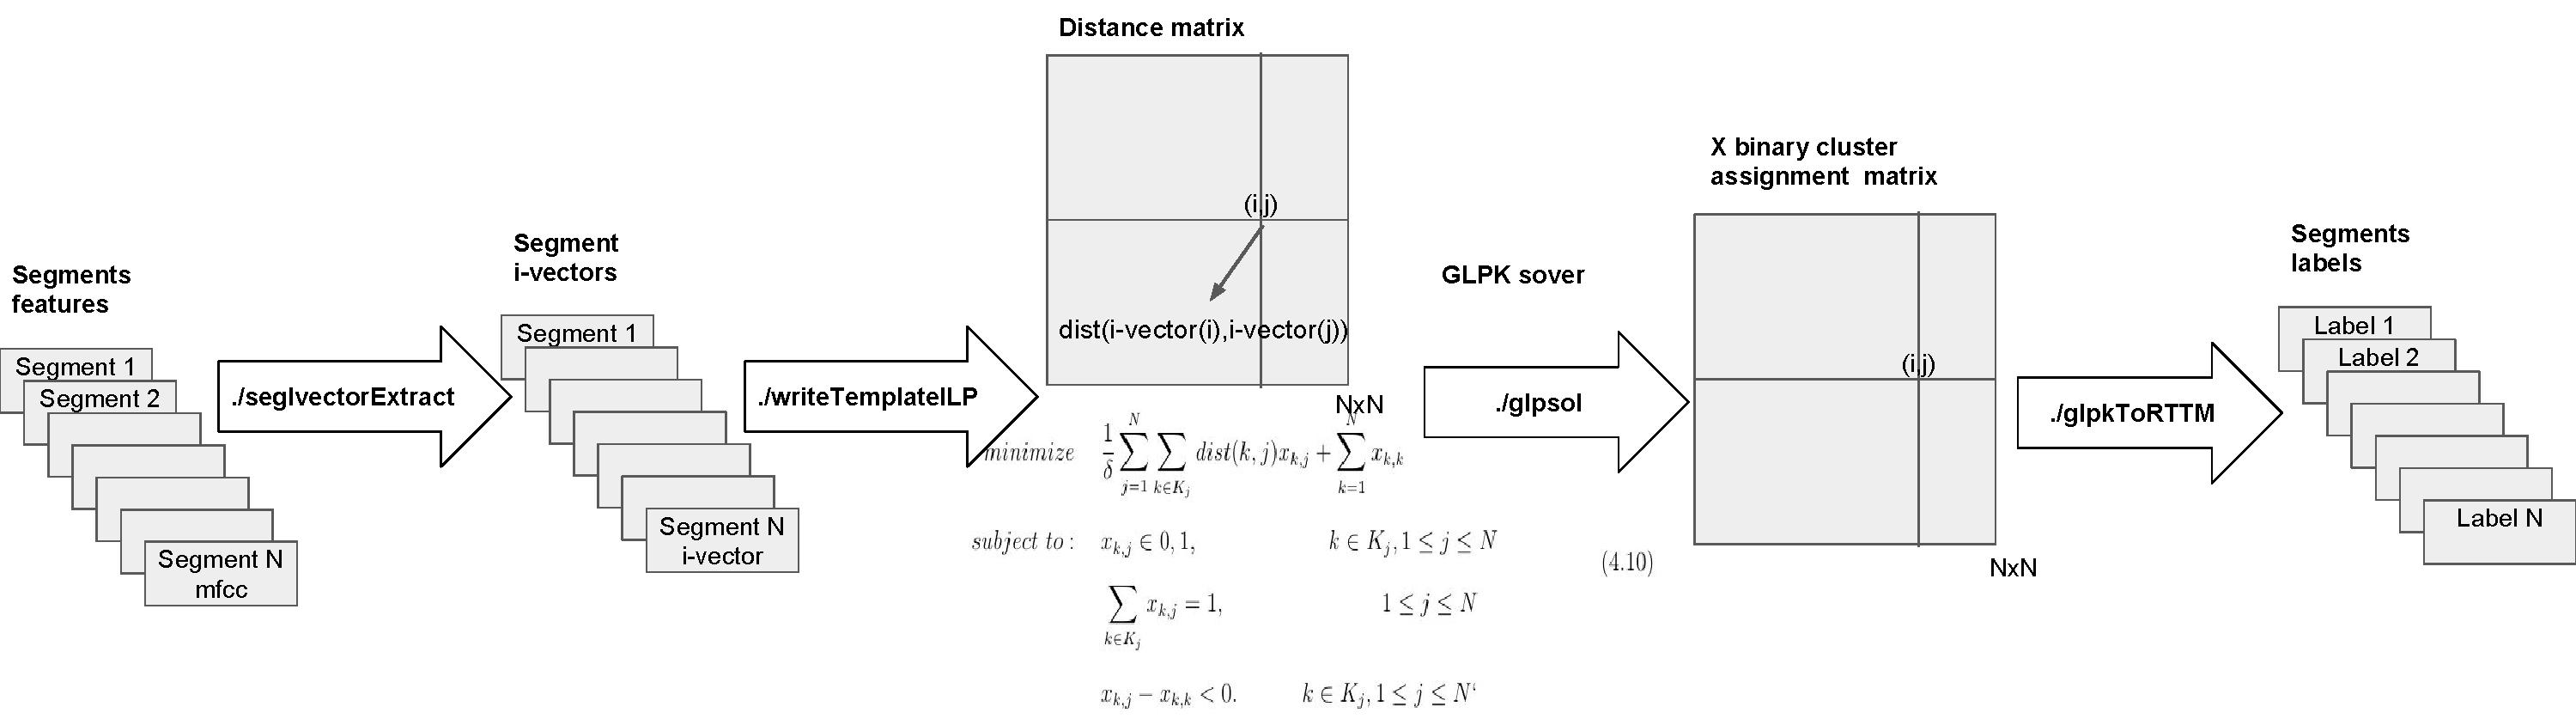
\includegraphics[height = 1.8in, width=1\textwidth]{figures/ilp_clustering_summary}
	\caption{\it \small Summary of ILP clustering using CRSSDiar. The binary executables used for each step is shown in the figure. }
	\label{fig:diarization_der}
	\vspace{-3mm}
\end{figure}


The descriptions provided in this section were based on existing studies~\cite{mueller2010ILP, rouvier2012ilp,dupuy2012ivectorsILP,dupuy2014ILPimprovement}. 
What was presented here was merely a brief of summary of existing publications. 
A novel addition in CRSSDiar has been in the choice of distance metric, $dist(.,.)$, described in the next section. 

\section{PLDA in ILP clustering}
\label{sec:plda_ilp}
Probabilistic linear discriminant analysis (PLDA) was thoroughly investigated in Chapter~\ref{chapter:backend} as a way to determine whether two individual [or groups of] i-vectors belong to the same speaker. 
The same question is faced during the clustering process for speaker diarization. 
Since ILP does not add any restrictions on the distance measures (see (\ref{eq:ilp_minimization_1})), PLDA can be used here as the distance metric, $dist(.,.)$. 
This creates a more appropriate setting for the clustering step, which aims to compare speaker identities across segments. 

The use of PLDA in speaker diarization has been proposed in a number of studies~\cite{prazak2011PLDAdrz, silovsky2011PLDAdrz, sell2014PLDAdrz}. 
PLDA proves especially useful in a class of speaker diarization problems that perform cross-session diarization. 
Cross-session diarization simultaneously clusters segments from several audio streams. 
In this scenario PLDA functions as a channel compensation algorithm. 
CRSSDiar proposes to use PLDA as a distance measure to perform global optimization in ILP clustering. 
This is expected to improve performance relative to Mahalanobis and cosine distances previously proposed for ILP clustering~\cite{dupuy2012ivectorsILP,dupuy2014ILPimprovement}. 

CRSSDiar accepts labeled background i-vectors to train a PLDA model (using Kaldi's PLDA class) to calculate distances. 
The function {\it computeDistanceMatrix}  calculates PLDA distances from segment i-vectors and background i-vectors in {\it writeTemplateILP}. 
In addition to {\it computeDistanceMatrix} for PLDA, CRSSDiar also calculates cosine distance, Mahalanobis distance, and conditional Bayes distance. 
Section~\ref{sec:other_distances_ilp}

\section{Other distance measures}
\label{sec:other_distances_ilp}
In addition to PLDA, three other 

\section{Evaluation}
\label{sec:chDrz_evaluation}
This section compares preliminary results from CRSSDiar, with existing results published by other diarization tool-kits. 
The experiments are conducted on the AMI meeting corpus, briefly described in Chapter~\ref{chapter:backend}. 
AMI consists of audio recordings from meetings, typically $30 min$ sessions. 
The corpus provides background additional information alongside the co-channel recordings, including individual speakers speech recorded from head-set and lapel microphones. 
In addition to audio files, the corpus contains segmentation ground-truth for speaker diarization. 
CRSSDiar uses this information to calculate diarization error rates for each session separately. 
The way CRSSDiar deals with different datasets is very similar to Kaldi. In that CRSSDiar binaries are independent of the data-set, but users can create recipe scripts that are specific to a particular corpus structure. 

\subsection{Diarization Error Rates}
\label{ssec:der}
The most popular error rate proposed for speaker diarization is diarization error rate (DER)~\cite{anguera2012DRZreview}. 
This error rate is a combination of three types of errors that can be made by a speaker diarization system: 
\begin{itemize}
	\item false alarm errors: segments that are falsely detected as speech segments. 
	\item miss errors: segments that contain speech from one of the speakers, but are missed (flagged non-speech) by the diarization system. 
	\item speaker error: the clustering error, which incorrectly labels segments. 
\end{itemize}

The last type of error is the most difficult to verify, since the diarization system has no prior knowledge of the speakers and therefore assigns its own labels to segments. 
So the labeling produced by the diarization system does not correspond to labels from ground-truth. The figure below shows an example this problem where the diarization system performs perfectly, but the labels it generates are different from ground-truth. 
Figure~\ref{fig:diarization_der} highlights the types of error that are made during diarization. 

\begin{figure}[h!]
	\centering
	\textbf{Speaker Diarization Errors}\par\medskip
	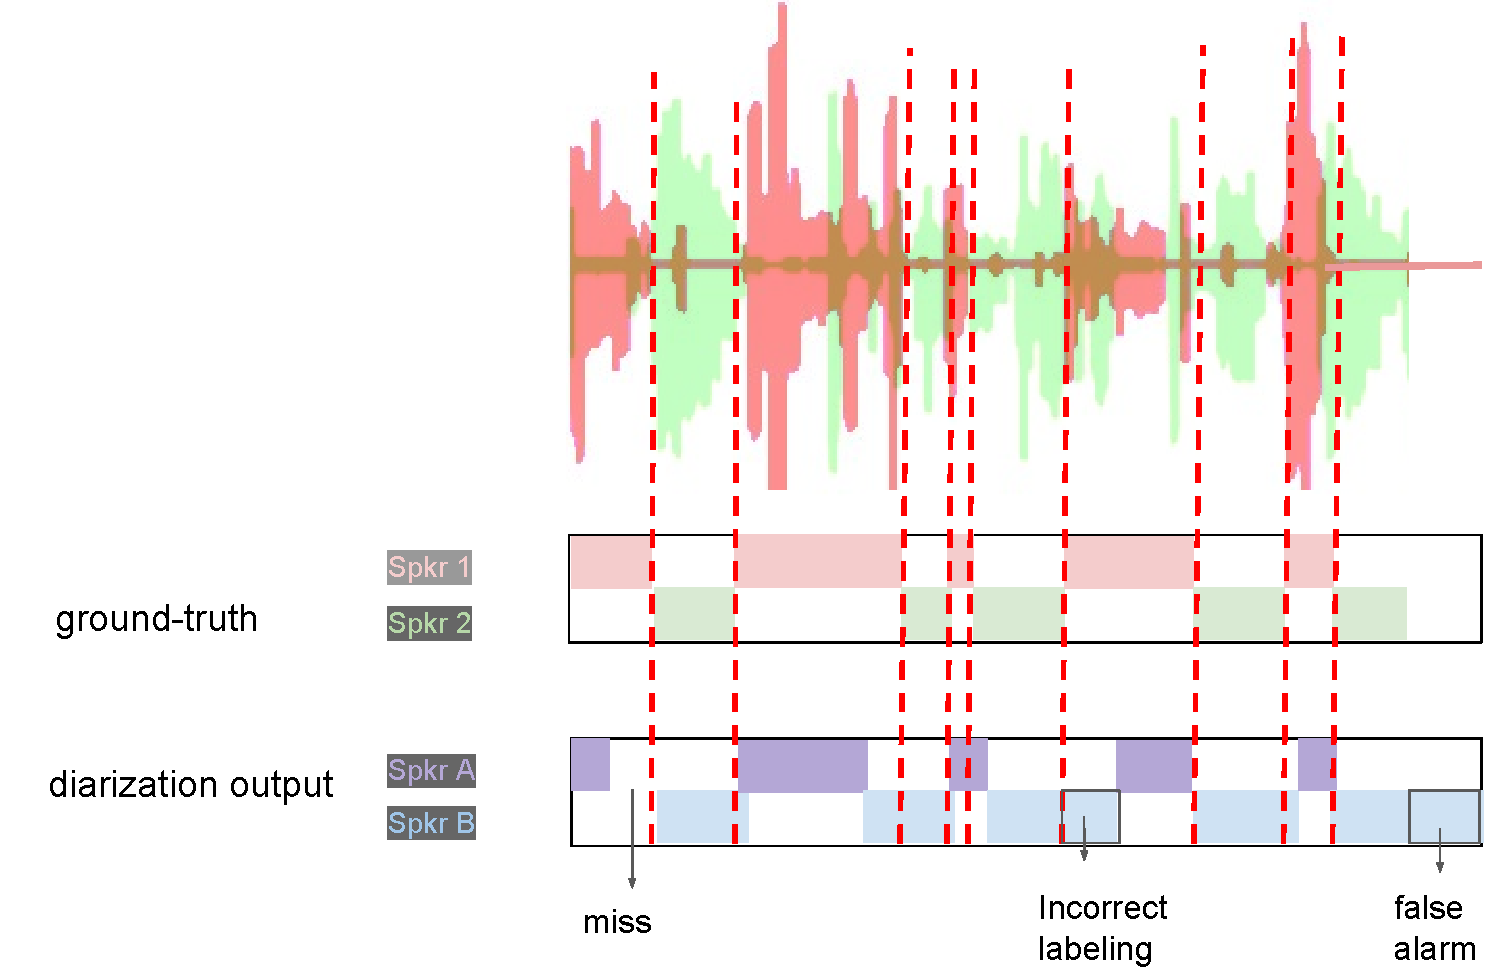
\includegraphics[height = 3in, width=1\textwidth]{figures/diarization_example_der}
	\caption{\it \small Shows three types of errors made by a diarization system. 1) false alarms: segment that does not contain speech is labeled by diarization system. 2) miss: segment containing speech is not labeled by diarization system. 
		3) incorrect labeling: the third type of error assumes that A is 1 and B is 2. It is up to the diarization error rate calculator to make this assignment.}
	\label{fig:diarization_der}
	\vspace{-3mm}
\end{figure}

It is also shown that the labels assigned by the speaker diarization system ($A, B$) are different from ground-truth labels ($1, 2$). 
It is up to the diarization error rate calculator to make decide that $A:1$ and $B:1$. 
This is done by considering all possibilities, in this case $(A:1,B:2)$ and $(A:2,B:2)$, and returning the assignment that results in minimum labeling error. 


The formulation proposed by NIST for diarization error rate\footnote{Unfortunately, NIST has removed the online evaluation plan from its website. The equations provided here are from Xavier Anguera's PhD thesis~\cite{anguera2007phd}.} is~\cite{anguera2012DRZreview}:
\begin{equation}
DER = E_{spkr} + E_{miss} + E_{fa}, 
\end{equation}
where: 
\begin{equation}
E_{spkr} = \frac{\sum\limits_{s=1}^{S} dur(s)(min(N_{groundtruth}(s),N_{diarization})-N_{correct}(s))}{T_{score}}
\end{equation}
\begin{equation}
E_{fa} = \frac{\sum\limits_{s=1}^S dur(s)(N_{diarization}(s)-N_{groundtruth}(s))}{T_{score}}
\end{equation}
\begin{equation}
E_{miss} = \frac{\sum\limits_{s=1}^S dur(s)(N_{groundtruth}(s) - N_{diarization}(s))}{T_{score}}
\end{equation}
in which $S$ is the total number of segments. $dur(s)$ is the duration of segment $s$. $N_{groundtruth}(s)$ is the number of speakers in segment $s$ provided by the ground-truth. 
$N_{diarization}(s)$ is the number of speakers in segment $s$ hypothesized by the diarization system. 
$N_{correct}(s)$ is the number of speakers correctly matched by the diarization system. 
Finally, $T_{score}$ is the total scoring time. 

CRSSDiar uses an evaluation Perl script provided by NIST that calculates DER alongside the individual errors described above. 
This script requires a certain input format for the labels, called RTTM. 
CRSSDiar contains labelToRTTM and glpkToRTTM binaries that convert Kaldi vectors to RTTM. 
In addition, the output of GLPK clustering module can be converted into RTTM using glpkToRTTM. 

 

 
